% ============================================================
% Final Project Presentation
% Project 20: Text Search within Images (OCR-based)
% Course: CSC15012 - Applications of NLP in Industry
% Student: Le Dinh Minh Quan - 23127460 - 23CNTThuc
% ============================================================

\documentclass[10pt,aspectratio=169]{beamer}

\mode<presentation>
{
  \usetheme{Madrid}
  \usecolortheme{seahorse}
  \usefonttheme{default}
  \setbeamertemplate{navigation symbols}{}
  \setbeamertemplate{caption}[numbered]
  \setbeamertemplate{footline}[frame number]
}

% ---- Packages ----
\usepackage[english]{babel}
\usepackage[utf8]{inputenc}
\usepackage{amsmath}
\usepackage{amssymb}
\usepackage{graphicx}
\usepackage{booktabs}
\usepackage{xcolor}
\usepackage{hyperref}
\usepackage{xurl}
\usepackage{tikz}
\usepackage{pgfplots}
\pgfplotsset{compat=1.18}
\usetikzlibrary{shapes.geometric, arrows.meta, positioning, fit, backgrounds, shadows}
\usepackage{listings}
\lstset{
  basicstyle=\ttfamily\scriptsize,
  breaklines=true,
  frame=single,
  backgroundcolor=\color{gray!10},
  keywordstyle=\color{blue},
  commentstyle=\color{green!60!black},
  stringstyle=\color{red!70!black},
  showstringspaces=false,
  tabsize=2
}

% ---- HCMUS LOGO ----
% Upload logo_hcmus.png to Overleaf to display the logo (top-right of every slide).
% If the file is missing, no logo is shown (no error).
\IfFileExists{logo_hcmus.png}{\logo{\includegraphics[height=0.7cm]{logo_hcmus.png}}}{}

% ---- TITLE METADATA ----
\title[Project 20: Text Search in Images]{Project 20: Text Search within Images (OCR-based)}
\subtitle{Hybrid BM25 + Dense Retriever + RRF over OCR text, with a 5-decision search agent}
\author[Le Dinh Minh Quan]{Le Dinh Minh Quan \\ \small ID: 23127460 -- Class: 23CNTThuc}
\institute[HCMUS]{Vietnam National University Ho Chi Minh City \\ University of Science -- Faculty of Information Technology \\ \small Course: CSC15012 -- Applications of NLP in Industry}
\date{2026}

\begin{document}

% ============================================================
% SLIDE 1: TITLE
% ============================================================
\begin{frame}
  \titlepage
\end{frame}

% ============================================================
% SLIDE 2: OUTLINE
% ============================================================
\begin{frame}{Outline}
\begin{columns}[T]
\begin{column}{0.5\textwidth}
\begin{enumerate}
  \item Business Problem \& Motivation
  \item Proposed NLP Solution \& Success Metrics
  \item System Architecture
  \item Repository \& Tech Stack
  \item Data Management \& Licenses
  \item Training / Autopilot Workflow
\end{enumerate}
\end{column}
\begin{column}{0.5\textwidth}
\begin{enumerate}
  \setcounter{enumi}{6}
  \item Evaluation Results \& Noise Sweep
  \item The 5-Decision Agent (D1--D5)
  \item Agent Example Interactions
  \item Deployment
  \item Ethics, Privacy \& Fairness
  \item Monitoring \& Continual Learning
  \item Key Takeaways \& Resources
\end{enumerate}
\end{column}
\end{columns}
\end{frame}

% ============================================================
% SLIDE 3: BUSINESS PROBLEM & MOTIVATION
% ============================================================
\begin{frame}{1. Business Problem \& Motivation}
\begin{block}{The question}
\textbf{``Which images literally CONTAIN this text?''} --- not \emph{what an image depicts}. E.g. \textit{find images containing the word \texttt{INVOICE}}; \textit{receipts mentioning a \texttt{2023} date}; \textit{the page with \texttt{PO-4471}}.
\end{block}

\begin{columns}[T]
\begin{column}{0.5\textwidth}
\textbf{Use cases (a pile of images)}
\begin{itemize}
  \item Document / receipt / invoice archives
  \item Scanned-contract \& compliance / e-discovery
  \item Screenshot \& photo-library search
\end{itemize}
\textbf{Why NLP?} OCR text is \emph{noisy} (\texttt{INVOICE}$\to$\texttt{INV0ICE}); a brittle exact-substring filter misses any term off by one character.
\end{column}
\begin{column}{0.5\textwidth}
\textbf{Distinct from P19 (CLIP, sibling)}
\begin{itemize}
  \item P19: visual/semantic --- query \& pixels share \emph{no} vocabulary
  \item \textbf{P20}: lexical --- query \& OCR text share the \emph{same} lexical space
  \item $\Rightarrow$ \textbf{BM25 is the LEAD signal}, not a baseline
\end{itemize}
\end{column}
\end{columns}
\end{frame}

% ============================================================
% SLIDE 4: PROPOSED NLP SOLUTION + SUCCESS METRICS
% ============================================================
\begin{frame}{2. Proposed NLP Solution \& Success Metrics}
\begin{block}{Solution}
OCR each image $\rightarrow$ per-image text ``document'' $\rightarrow$ \textbf{hybrid BM25 + dense (trained) + RRF} index $\rightarrow$ \textbf{verify} the term literally appears (fuzzy-tolerant) $\rightarrow$ \textbf{snippet} + \textbf{abstain} if none. A deterministic D1--D5 agent orchestrates it.
\end{block}

\begin{table}[h]
\centering\small
\begin{tabular}{lll}
\toprule
\textbf{Type} & \textbf{Metric} & \textbf{Target} \\
\midrule
Retrieval (primary) & Recall@\{1,5,10\}, MRR & high; $R@1\le R@5\le R@10$ \\
Verification & Exact-Match precision@K & match BM25's ceiling \\
OCR quality & CER / WER (searchability cap) & low; reported together \\
Behaviour & Abstain on a nonexistent term & must abstain, not guess \\
\bottomrule
\end{tabular}
\end{table}

\textbf{Small trained surface, large deterministic core}: exactly \textbf{one} model is trained --- the dense retriever (\texttt{bge-small-en-v1.5}, MIT). OCR, BM25, RRF, the verifier, and the agent are pretrained/algorithmic.
\end{frame}

% ============================================================
% SLIDE 5: SYSTEM ARCHITECTURE (TikZ)
% ============================================================
\begin{frame}{3. System Architecture}
\centering
\resizebox{\linewidth}{!}{%
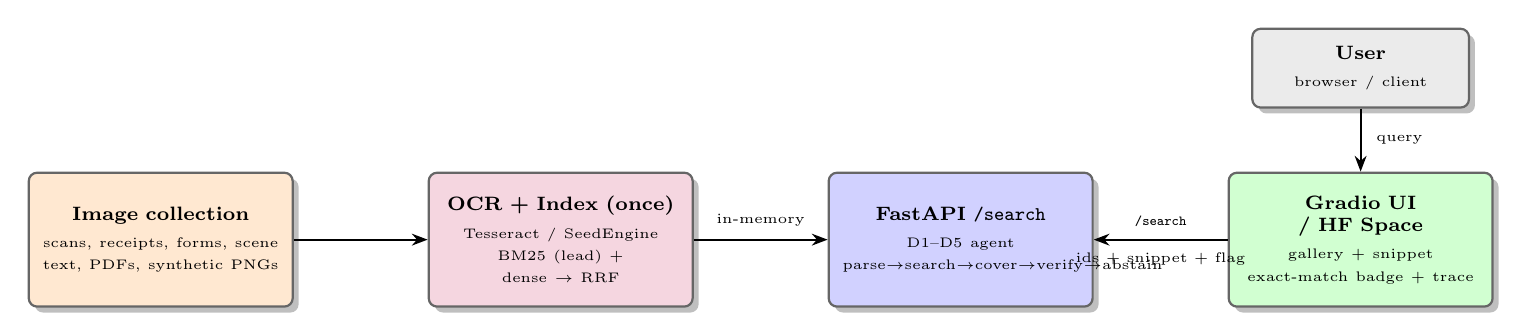
\begin{tikzpicture}[
  node distance=0.9cm and 1.7cm,
  box/.style={rectangle, draw=black!60, rounded corners=3pt, thick,
              text width=3.0cm, minimum height=1.7cm, align=center,
              inner sep=5pt, font=\scriptsize, drop shadow},
  ocrbox/.style={box, fill=purple!16},
  idxbox/.style={box, fill=orange!18},
  apibox/.style={box, fill=blue!18},
  uibox/.style={box, fill=green!18},
  userbox/.style={box, fill=gray!16, text width=2.4cm, minimum height=1.0cm},
  arrow/.style={-{Stealth[length=2mm]}, thick}
]
\node[idxbox] (coll) {%
  \textbf{Image collection}\\[2pt]
  {\tiny scans, receipts, forms, scene text, PDFs, synthetic PNGs}
};
\node[ocrbox, right=of coll] (ocr) {%
  \textbf{OCR + Index (once)}\\[2pt]
  {\tiny Tesseract / SeedEngine}\\
  {\tiny BM25 (lead) + dense $\to$ RRF}
};
\node[apibox, right=of ocr] (api) {%
  \textbf{FastAPI \texttt{/search}}\\[2pt]
  {\tiny D1--D5 agent}\\
  {\tiny parse$\to$search$\to$cover$\to$verify$\to$abstain}
};
\node[uibox, right=of api] (ui) {%
  \textbf{Gradio UI / HF Space}\\[2pt]
  {\tiny gallery + snippet}\\
  {\tiny exact-match badge + trace}
};
\node[userbox, above=0.8cm of ui] (user) {%
  \textbf{User}\\[2pt]
  {\tiny browser / client}
};
\draw[arrow] (coll.east) -- (ocr.west);
\draw[arrow] (ocr.east) -- node[above=1pt, font=\tiny, midway] {in-memory} (api.west);
\draw[arrow] (ui.west) -- node[above=1pt, font=\tiny, midway] {\texttt{/search}} node[below=1pt, font=\tiny, midway] {ids + snippet + flag} (api.east);
\draw[arrow] (user) -- node[right=2pt, font=\tiny] {query} (ui);
\end{tikzpicture}%
}

\vspace{0.2cm}
\scriptsize Collection \textbf{OCR-indexed once at startup}, held in memory. A query never triggers OCR --- only the short query string is encoded. CPU-first: OCR + BM25 + RRF + agent on CPU; only the dense arm (and optional rerank/byt5) use a GPU if present. \texttt{IMGTS\_DENSE\_ENABLED=0} $\Rightarrow$ strong BM25-only mode.
\end{frame}

% ============================================================
% SLIDE 6: REPOSITORY & TECH STACK
% ============================================================
\begin{frame}[fragile]{4. Repository Structure \& Tech Stack}
\begin{columns}[T]
\begin{column}{0.56\textwidth}
\textbf{GitHub repo} (public, MIT) \\
\scriptsize \url{https://github.com/ledinhminhquan/20_Text_Search_in_Images}

\vspace{0.12cm}
\begin{lstlisting}[basicstyle=\ttfamily\tiny]
src/imgtextsearch/
  config.py cli.py logging_utils.py
  ocr/        engine.py    # Tesseract/SeedEngine/Stub
  data/       synth_text_images.py samples.py
  models/     encoder.py baseline.py registry
  index/      text_index.py lexical.py # BM25+dense+RRF
  training/   train_retriever.py evaluate.py tune.py
  agent/      search_agent.py tools.py policy.py state.py
  api/        main.py schemas.py ui.py
  analysis/   error_analysis.py latency.py
  autoreport/ report_pdf.py slides_pptx.py
  monitoring/ drift_report.py
  automation/ autopilot.py   grading/ checklist.py
docs/ (14 Section-I docs)  notebooks/  tests/  deploy/
\end{lstlisting}
\end{column}
\begin{column}{0.44\textwidth}
\textbf{Tech stack (all MIT/Apache)}
\begin{itemize}\scriptsize
  \item Python (numpy, Pillow, pydantic)
  \item \textbf{Tesseract} (Apache) + offline SeedEngine
  \item \textbf{\texttt{bge-small-en-v1.5}} (MIT, trained core)
  \item pure-python \textbf{BM25} (lead) + \textbf{RRF} ($c{=}60$)
  \item PyMuPDF born-digital router
  \item FastAPI + Uvicorn; Gradio
  \item Docker (tesseract + fonts + libGL)
  \item Hugging Face Space
  \item Colab / NVIDIA H100 autopilot
\end{itemize}
\textbf{Upgrades}: TrOCR / PP-OCRv5 OCR; \texttt{bge-base}; cross-encoder rerank; \texttt{byt5-small} post-OCR fix.
\end{column}
\end{columns}
\end{frame}

% ============================================================
% SLIDE 7: DATA MANAGEMENT & LICENSES
% ============================================================
\begin{frame}{5. Data Management \& Licenses}
\begin{columns}[T]
\begin{column}{0.5\textwidth}
\textbf{PRIMARY = synthetic generator}
\begin{itemize}\scriptsize
  \item No public ``find image containing X'' benchmark exists $\Rightarrow$ \textbf{synthesize one}
  \item Needle vocab (\texttt{INVOICE}, \texttt{PO-4471}, dates, amounts) + fillers
  \item Gold text embedded in each PNG (\texttt{imgsearch\_spec}); \textbf{gold map is OCR-independent}
  \item \texttt{\_noisify} rate $=$ the CER/WER knob
  \item Runs offline: \textbf{no Tesseract / torch / network}
\end{itemize}
\end{column}
\begin{column}{0.5\textwidth}
\textbf{Real corpora --- license posture}
\begin{table}[h]
\centering\scriptsize
\begin{tabular}{lll}
\toprule
\textbf{Dataset} & \textbf{License} & \textbf{Ship?} \\
\midrule
TextOCR\_OCR (112.7K) & MIT & demo \\
IIIT5K\_OCR (5.5K) & MIT & demo \\
cord-v2 (1.0K) & CC-BY-4.0 & demo (attrib.) \\
Post-OCR-Corr. (50.4K) & CC0 & demo \\
\midrule
docvqa\_1200 & unspec. & \textbf{FLAG} \\
funsd-layoutlmv3 & unspec. & \textbf{FLAG} \\
rvl\_cdip (400K) & other (NC) & \textbf{FLAG} \\
COCO-Text (\textasciitilde16K) & unspec. & \textbf{FLAG} \\
\bottomrule
\end{tabular}
\end{table}
\scriptsize Ship on \textbf{MIT + CC0 + CC-BY-4.0 + synthetic} only; gate every NC/unspecified set behind \texttt{research\_only}. \textbf{Surya} OCR (CC-BY-NC-SA) excluded from the default stack.
\end{column}
\end{columns}
\end{frame}

% ============================================================
% SLIDE 8: TRAINING / AUTOPILOT WORKFLOW
% ============================================================
\begin{frame}{6. Training / Autopilot Workflow (one-button Colab/H100)}
\centering
\begin{tikzpicture}[
  node distance=0.16cm,
  step/.style={rectangle, draw=black!60, rounded corners=2pt, thick,
              minimum width=11.6cm, minimum height=0.52cm, align=center, font=\scriptsize},
  setup/.style={step, fill=gray!15},
  data/.style={step, fill=purple!12},
  train/.style={step, fill=orange!15},
  eval/.style={step, fill=blue!15},
  deploy/.style={step, fill=green!15},
  arrow/.style={-{Stealth[length=1.8mm]}, thick}
]
\node[setup] (s1) {\textbf{1. Setup}: clone repo, \texttt{pip install .[all]}, set artifacts dir};
\node[data, below=of s1] (s2) {\textbf{2. Synthetic data (PRIMARY)}: render needle/filler pages, embed gold spec, record gold map};
\node[data, below=of s2] (s3) {\textbf{3. OCR + index}: \texttt{engine='auto'} (SeedEngine offline / Tesseract on Colab) $\to$ BM25 + dense};
\node[train, below=of s3] (s4) {\textbf{4. Fine-tune retriever}: \texttt{bge-small} MNRL on \texttt{(query, OCR-text)} pairs};
\node[eval, below=of s4] (s5) {\textbf{5. Evaluation}: Recall/MRR/rank, CER/WER, Exact-Match P@K vs baselines};
\node[eval, below=of s5] (s6) {\textbf{6. Noise sweep + error analysis}: CER knob $\to$ BM25 collapse vs hybrid+verify resilience};
\node[deploy, below=of s6] (s7) {\textbf{7. Auto-gen} report PDF + slides PPTX};
\node[deploy, below=of s7] (s8) {\textbf{8. Grade + bundle}: rubric self-check (target score 1.0)};
\node[deploy, below=of s8] (s9) {\textbf{9. Serve (optional)}: \texttt{serve --ui} (FastAPI :8000 + Gradio :8000/ui); Docker; HF Space};
\foreach \a/\b in {s1/s2,s2/s3,s3/s4,s4/s5,s5/s6,s6/s7,s7/s8,s8/s9}
  \draw[arrow] (\a) -- (\b);
\end{tikzpicture}

\vspace{0.12cm}
\scriptsize The same \texttt{engine='auto'} code path runs offline (SeedEngine) and on Colab/H100 (real Tesseract \texttt{image\_to\_data}), so CER/WER stay honest across both. The synthetic generator (step 2) unblocks everything with zero heavy deps.
\end{frame}

% ============================================================
% SLIDE 9: EVALUATION RESULTS & NOISE SWEEP
% ============================================================
\begin{frame}{7. Evaluation --- Verified Offline Seed + Noise Sweep}
\begin{columns}[T]
\begin{column}{0.48\textwidth}
\textbf{Verified offline (no torch/tesseract/network)}
\begin{table}[h]
\centering\scriptsize
\begin{tabular}{ll}
\toprule
\textbf{Quantity} & \textbf{Result} \\
\midrule
Recall@1 (unique codes) & \textbf{1.0} \\
MRR (unique codes) & \textbf{1.0} \\
Snippet highlighting & span returned \\
Absent term \texttt{zzqwx} & \textbf{ABSTAINS} \\
Agent decisions D1--D5 & \textbf{all 5 fire} \\
\bottomrule
\end{tabular}
\end{table}
\scriptsize \textbf{Read correctly}: $R@1{=}\text{MRR}{=}1.0$ is the \emph{expected} exact-term ceiling for unique clean codes (BM25 is faithful by construction). The trained dense arm's job is to \textbf{hold Recall up as CER rises} and on paraphrases, while the verifier holds Exact-Match precision at BM25's level.
\end{column}
\begin{column}{0.52\textwidth}
\textbf{OCR-noise sweep (illustrative shape)}
\begin{center}
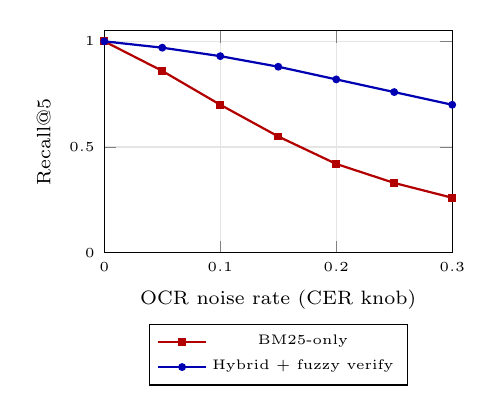
\begin{tikzpicture}
\begin{axis}[
  width=6.0cm, height=4.4cm,
  xlabel={\scriptsize OCR noise rate (CER knob)},
  ylabel={\scriptsize Recall@5},
  xmin=0, xmax=0.30, ymin=0, ymax=1.05,
  xtick={0,0.1,0.2,0.3}, ytick={0,0.5,1.0},
  tick label style={font=\tiny},
  label style={font=\tiny},
  legend style={font=\tiny, at={(0.5,-0.32)}, anchor=north, legend columns=1},
  grid=both, grid style={gray!20},
  every axis plot/.append style={thick}
]
\addplot[color=red!70!black, mark=square*, mark size=1pt] coordinates {(0,1.0)(0.05,0.86)(0.10,0.70)(0.15,0.55)(0.20,0.42)(0.25,0.33)(0.30,0.26)};
\addplot[color=blue!70!black, mark=*, mark size=1pt] coordinates {(0,1.0)(0.05,0.97)(0.10,0.93)(0.15,0.88)(0.20,0.82)(0.25,0.76)(0.30,0.70)};
\legend{BM25-only, Hybrid + fuzzy verify}
\end{axis}
\end{tikzpicture}
\end{center}
\scriptsize As OCR noise rises, BM25-only collapses (one char flip removes the literal token), while hybrid + bounded-fuzzy verify stays resilient: dense embeds \texttt{INV0ICE}$\approx$\texttt{INVOICE}, D4 confirms within edit distance~1. Baselines: BM25-only / dense-only / random.
\end{column}
\end{columns}
\end{frame}

% ============================================================
% SLIDE 10: THE 5-DECISION AGENT
% ============================================================
\begin{frame}{8. Agentic AI Component --- Deterministic D1--D5}
\centering
\begin{tikzpicture}[
  node distance=0.18cm,
  step/.style={rectangle, draw=black!60, rounded corners=2pt, thick,
              text width=11.4cm, minimum height=0.6cm, align=center, font=\scriptsize, inner sep=4pt},
  parse/.style={step, fill=gray!15},
  search/.style={step, fill=blue!15},
  cover/.style={step, fill=red!12},
  verify/.style={step, fill=orange!16},
  final/.style={step, fill=green!15},
  arrow/.style={-{Stealth[length=2mm]}, thick}
]
\node[parse] (d1) {\textbf{D1 Parse + classify} (\textbf{tool}): intent \texttt{exact\_code}/\texttt{keyword}/\texttt{phrase}; empty/short $\to$ \textbf{ABSTAIN\_EARLY}};
\node[search, below=of d1] (d2) {\textbf{D2 Search} (\textbf{tool}): BM25 (lead) + dense \texttt{bge-small} $\to$ \textbf{RRF} ($c{=}60$) $\to$ top-$k$; carry \emph{raw} signals};
\node[cover, below=of d2] (d3) {\textbf{D3 Coverage} (\textbf{reasoning}): gate on \textbf{RAW} BM25 hits + \textbf{RAW} cosine (never fused); weak $\to$ \textbf{WIDEN once}};
\node[verify, below=of d3] (d4) {\textbf{D4 Literal verify + snippet} (\textbf{decision}): exact / fuzzy ($\le1$ edit); \texttt{exact\_intent} \& none $\to$ \textbf{DROP} FP};
\node[final, below=of d4] (d5) {\textbf{D5 Finalize / abstain} (\textbf{decision}): 0 verified $\to$ \textbf{ABSTAIN} ``not found''; else ranked + snippets + labels};
\foreach \a/\b in {d1/d2,d2/d3,d3/d4,d4/d5}
  \draw[arrow] (\a) -- (\b);
\draw[arrow] (d3.east) to[out=0,in=0] node[right, font=\tiny] {widen $\le1$} (d2.east);
\end{tikzpicture}

\vspace{0.12cm}
\scriptsize \textbf{Value-add over blind semantic ranking}: (1) literal verification drops semantic false-positives; (2) snippet + word bbox + OCR confidence; (3) honest abstention. \textbf{P08/P18 gotcha avoided}: D3 gates on \textbf{raw} signals, not the fused RRF score (which always looks confident). Every gate writes a replayable \texttt{ToolTrace}. Optional LLM brain is \textbf{OFF by default}, advisory-only, never changes ranking.
\end{frame}

% ============================================================
% SLIDE 11: AGENT EXAMPLE INTERACTIONS
% ============================================================
\begin{frame}[fragile]{9. Agent Example Interactions}
\textbf{Example 1 --- Happy path: unique code exists $\rightarrow$ FINALIZE}
\begin{lstlisting}[basicstyle=\ttfamily\tiny]
Query: PO-4471
D2  BM25 fires on page_0042 (high-IDF) score=8.91; dense cosine=0.62 -> RRF shortlist
D3  n_bm25_hits=1 (>=1) AND cosine 0.62 >= tau_soft 0.55 -> STRONG
D4  page_0042: "po-4471" EXACT -> VERIFIED; snippet="...REF [PO-4471] TOTAL $1,250.00..."
    page_0117/page_0008: not present, exact_intent -> DROP (semantic false-positive)
D5  FINALIZE: [ page_0042 | snippet | bbox | high ]   needs_review=False
\end{lstlisting}

\textbf{Example 2 --- OCR noise: fuzzy match earns its keep $\rightarrow$ FINALIZE (flagged)}
\begin{lstlisting}[basicstyle=\ttfamily\tiny]
Query: INVOICE   (page_0091 OCR'd as "INV0ICE", O->0)
D2  BM25: "invoice" != "inv0ice" -> n_bm25_hits=0; dense cosine=0.71 -> shortlist top=page_0091
D3  n_bm25_hits=0 BUT cosine 0.71 >= tau_soft 0.55 -> STRONG (cosine arm)
D4  exact FAILS; edit_distance("invoice","inv0ice")=1 <= 1 -> VERIFIED(fuzzy); flag fuzzy_match
D5  FINALIZE FLAGGED: [ page_0091 | medium | fuzzy_match | needs_review=True ]
\end{lstlisting}

\textbf{Example 3 --- Term not in collection $\rightarrow$ ABSTAIN}
\begin{lstlisting}[basicstyle=\ttfamily\tiny]
Query: zzqwx
D2  BM25: 0 hits; dense cosine=0.22 (nearest junk)
D3  cosine 0.22 < tau_floor 0.35 AND n_bm25_hits=0 -> jump to D5 ABSTAIN
D5  ABSTAIN: "not found in any image"  needs_review=True
    (high-looking RRF fused top score correctly IGNORED -- D3 gated on RAW cosine)
\end{lstlisting}
\end{frame}

% ============================================================
% SLIDE 12: DEPLOYMENT
% ============================================================
\begin{frame}[fragile]{10. Deployment (deployable; not on a live public URL)}
\textbf{Four formats delivered}
\begin{itemize}\small
  \item \textbf{REST API} (FastAPI): \texttt{GET /healthz}, \texttt{GET /stats}, \texttt{POST /search}, \texttt{POST /reindex} (admin, OFF)
  \item \textbf{CLI}: \texttt{imgtextsearch demo-agent / search / evaluate / autopilot / grade / serve --ui}
  \item \textbf{Docker}: \texttt{Dockerfile} (tesseract-ocr + fonts + libGL) + \texttt{docker-compose.yml}
  \item \textbf{Gradio UI + HF Space}: query $\to$ gallery + highlighted snippets + exact-match badge + trace panel
\end{itemize}

\begin{lstlisting}[basicstyle=\ttfamily\tiny]
POST /search {"query":"INVOICE","top_k":5,"fuzzy":true}
{ "query":"invoice","abstained":false,"needs_review":false,
  "results":[ {"image_id":"page_0042.png","score":0.0328,"exact_match":true,
               "snippet":"CUSTOMER 1187 **INVOICE** DATE 2023-04-12","confidence_label":"high"},
              {"image_id":"page_0117.png","exact_match":false,"fuzzy_match":true,
               "snippet":"TOTAL 1,250.00 **INV0ICE** NO PO-4471","confidence_label":"medium"} ],
  "trace":[ ...D1..D5... ], "latency_ms":23.7 }     # abstain (zzqwx) -> 200, results:[], needs_review:true
\end{lstlisting}

\scriptsize \textbf{CPU-first}: OCR + BM25 + RRF + agent + verifier on CPU; only dense (+optional rerank/byt5) use a GPU if present. Cold start is OCR-bound $\Rightarrow$ ship a pre-built index artifact for large collections; \texttt{/healthz} readiness tolerates a long cold start. A query never triggers OCR.
\end{frame}

% ============================================================
% SLIDE 13: ETHICS, PRIVACY & FAIRNESS
% ============================================================
\begin{frame}{11. Ethics, Privacy \& Fairness}
\begin{columns}[T]
\begin{column}{0.5\textwidth}
\textbf{Privacy --- a search engine over a doc trove}
\begin{itemize}\small
  \item Index can hold PII / IDs / financial / medical text
  \item \textbf{No query retention} by default; LLM brain \textbf{OFF}
  \item Consent + access control \emph{before} indexing
  \item PII redaction before indexing (word boxes enable it)
  \item Deterministic \texttt{ToolTrace} $\Rightarrow$ auditable
\end{itemize}
\textbf{Robustness}: OCR-error false negatives recovered by dense+RRF+fuzzy verify; index scaling via ANN swap; fail-soft to BM25-only.
\end{column}
\begin{column}{0.5\textwidth}
\textbf{OCR-quality bias $\Rightarrow$ unequal recall}
\begin{itemize}\small
  \item Findable only if OCR reads it right
  \item Varies by script/language, font, scan quality
  \item \textbf{Measured \& reported}: CER/WER per script/scan-quality, not one aggregate
  \item English is the supported target; non-EN is research-only --- \textbf{no equal-multilingual claim}
\end{itemize}
\textbf{High-stakes false negatives}: \textbf{abstain $\ne$ proof of absence}. Tool surfaces a snippet for \emph{human} confirmation; low-confidence results explicitly flagged, never silent.
\end{column}
\end{columns}
\end{frame}

% ============================================================
% SLIDE 14: MONITORING & CONTINUAL LEARNING
% ============================================================
\begin{frame}{12. Monitoring \& Continual Learning}
\begin{columns}[T]
\begin{column}{0.5\textwidth}
\textbf{Monitoring (from the trace, no gold)}
\begin{itemize}\small
  \item Abstain rate, fuzzy-match rate (CER proxy)
  \item Exact-match rate, top \textbf{raw} cosine drift (earliest retriever-drift signal)
  \item Widen rate, low-confidence / excluded count
  \item Per-stage latency p50/p95/p99
\end{itemize}
\textbf{Three drift channels watched separately}: query drift, document drift, OCR-quality drift $\Rightarrow$ the right fix fires (retrain vs re-OCR vs index update).
\end{column}
\begin{column}{0.5\textwidth}
\textbf{Continual learning}
\begin{enumerate}\small
  \item Incremental ingest appends to both arms (\emph{no retrain})
  \item Re-OCR on engine upgrade (provenance fingerprint)
  \item Feedback $\to$ hard positives / hard negatives (MNRL)
  \item Guard: never train to ``find'' a term not in the OCR text
  \item \textbf{Gated promotion}: must not regress Recall/MRR \emph{and} must not lower Exact-Match P@K
\end{enumerate}
\textbf{Rollback} to BM25-only is a strong literal-search floor $\Rightarrow$ low-risk retriever rollouts.
\end{column}
\end{columns}
\end{frame}

% ============================================================
% SLIDE 15: KEY TAKEAWAYS & RESOURCES (final slide)
% ============================================================
\begin{frame}{13. Key Takeaways \& Resources}
\textbf{Key takeaways}
\begin{itemize}\small
  \item Complete end-to-end OCR document-search: OCR $\to$ text index $\to$ BM25+dense+RRF $\to$ verify+snippet $\to$ abstain
  \item Exactly \textbf{one} trained component (\texttt{bge-small-en-v1.5}, MIT, MNRL); \textbf{BM25 is the lead arm}, not a baseline
  \item Deterministic 5-decision agent: literal verification + snippet highlighting + abstention; gates on \textbf{raw} signals; replayable \texttt{ToolTrace}
  \item \textbf{Verified offline}: $R@1{=}\text{MRR}{=}1.0$ on unique codes, snippet highlight, correct \texttt{zzqwx} abstention, all 5 decisions fire
  \item Deployable: FastAPI + Gradio + Docker + HF Space + one-button Colab/H100 autopilot; default stack fully MIT/Apache
\end{itemize}

\textbf{Future work}: active learning from feedback hard pairs; neural OCR/retriever upgrades (TrOCR/PP-OCRv5, \texttt{bge-base}, rerank, byt5); ANN index for 400K-scale; per-subset fairness reporting; live public Space hosting.

\begin{block}{Resources}
\centering
\small \textbf{GitHub (public, MIT)}: \url{https://github.com/ledinhminhquan/20_Text_Search_in_Images}
\end{block}

\vspace{0.15cm}
\centering
\Large\textbf{Thank you for your attention!}\\[0.15cm]
\normalsize Le Dinh Minh Quan -- 23127460 -- 23CNTThuc \\
\small CSC15012 -- Applications of NLP in Industry -- 2026
\end{frame}

\end{document}
